\section{Introduction}
\label{sec:intro}

Large Language Models (LLMs) have enabled increasingly capable autonomous agents that can reason, use tools, interact with environments, and complete complex tasks ranging from software engineering to web navigation~\citep{yao2023react,zhang2024codeagent,he2024webvoyager}. 
%
Beyond the foundation model, the empirical performance of an agent is fundamentally governed by the surrounding \emph{agent harness}~\citep{yang2024opro,khattab2024dspy,agrawal2026gepa}. 
%
The same frozen model can exhibit substantially different performance under different system prompts, injected knowledge, tool interfaces, control loops, recovery mechanisms, and runtime configurations. 
%
Unlike model weights, which may be closed, rented, or prohibitively expensive to update, the harness is often the only component that can be modified during deployment. 
%
Yet harnesses remain largely hand-engineered, making their development difficult to scale as models, tools, and application environments rapidly evolve. This motivates \emph{agent-harness self-evolution}~\citep{ren2026selfimprovementsmodernagenticsystems}, which aims to enable an agent to diagnose its own failures and iteratively improve its harness without updating the underlying model.

\begin{figure}[t]
  \centering
  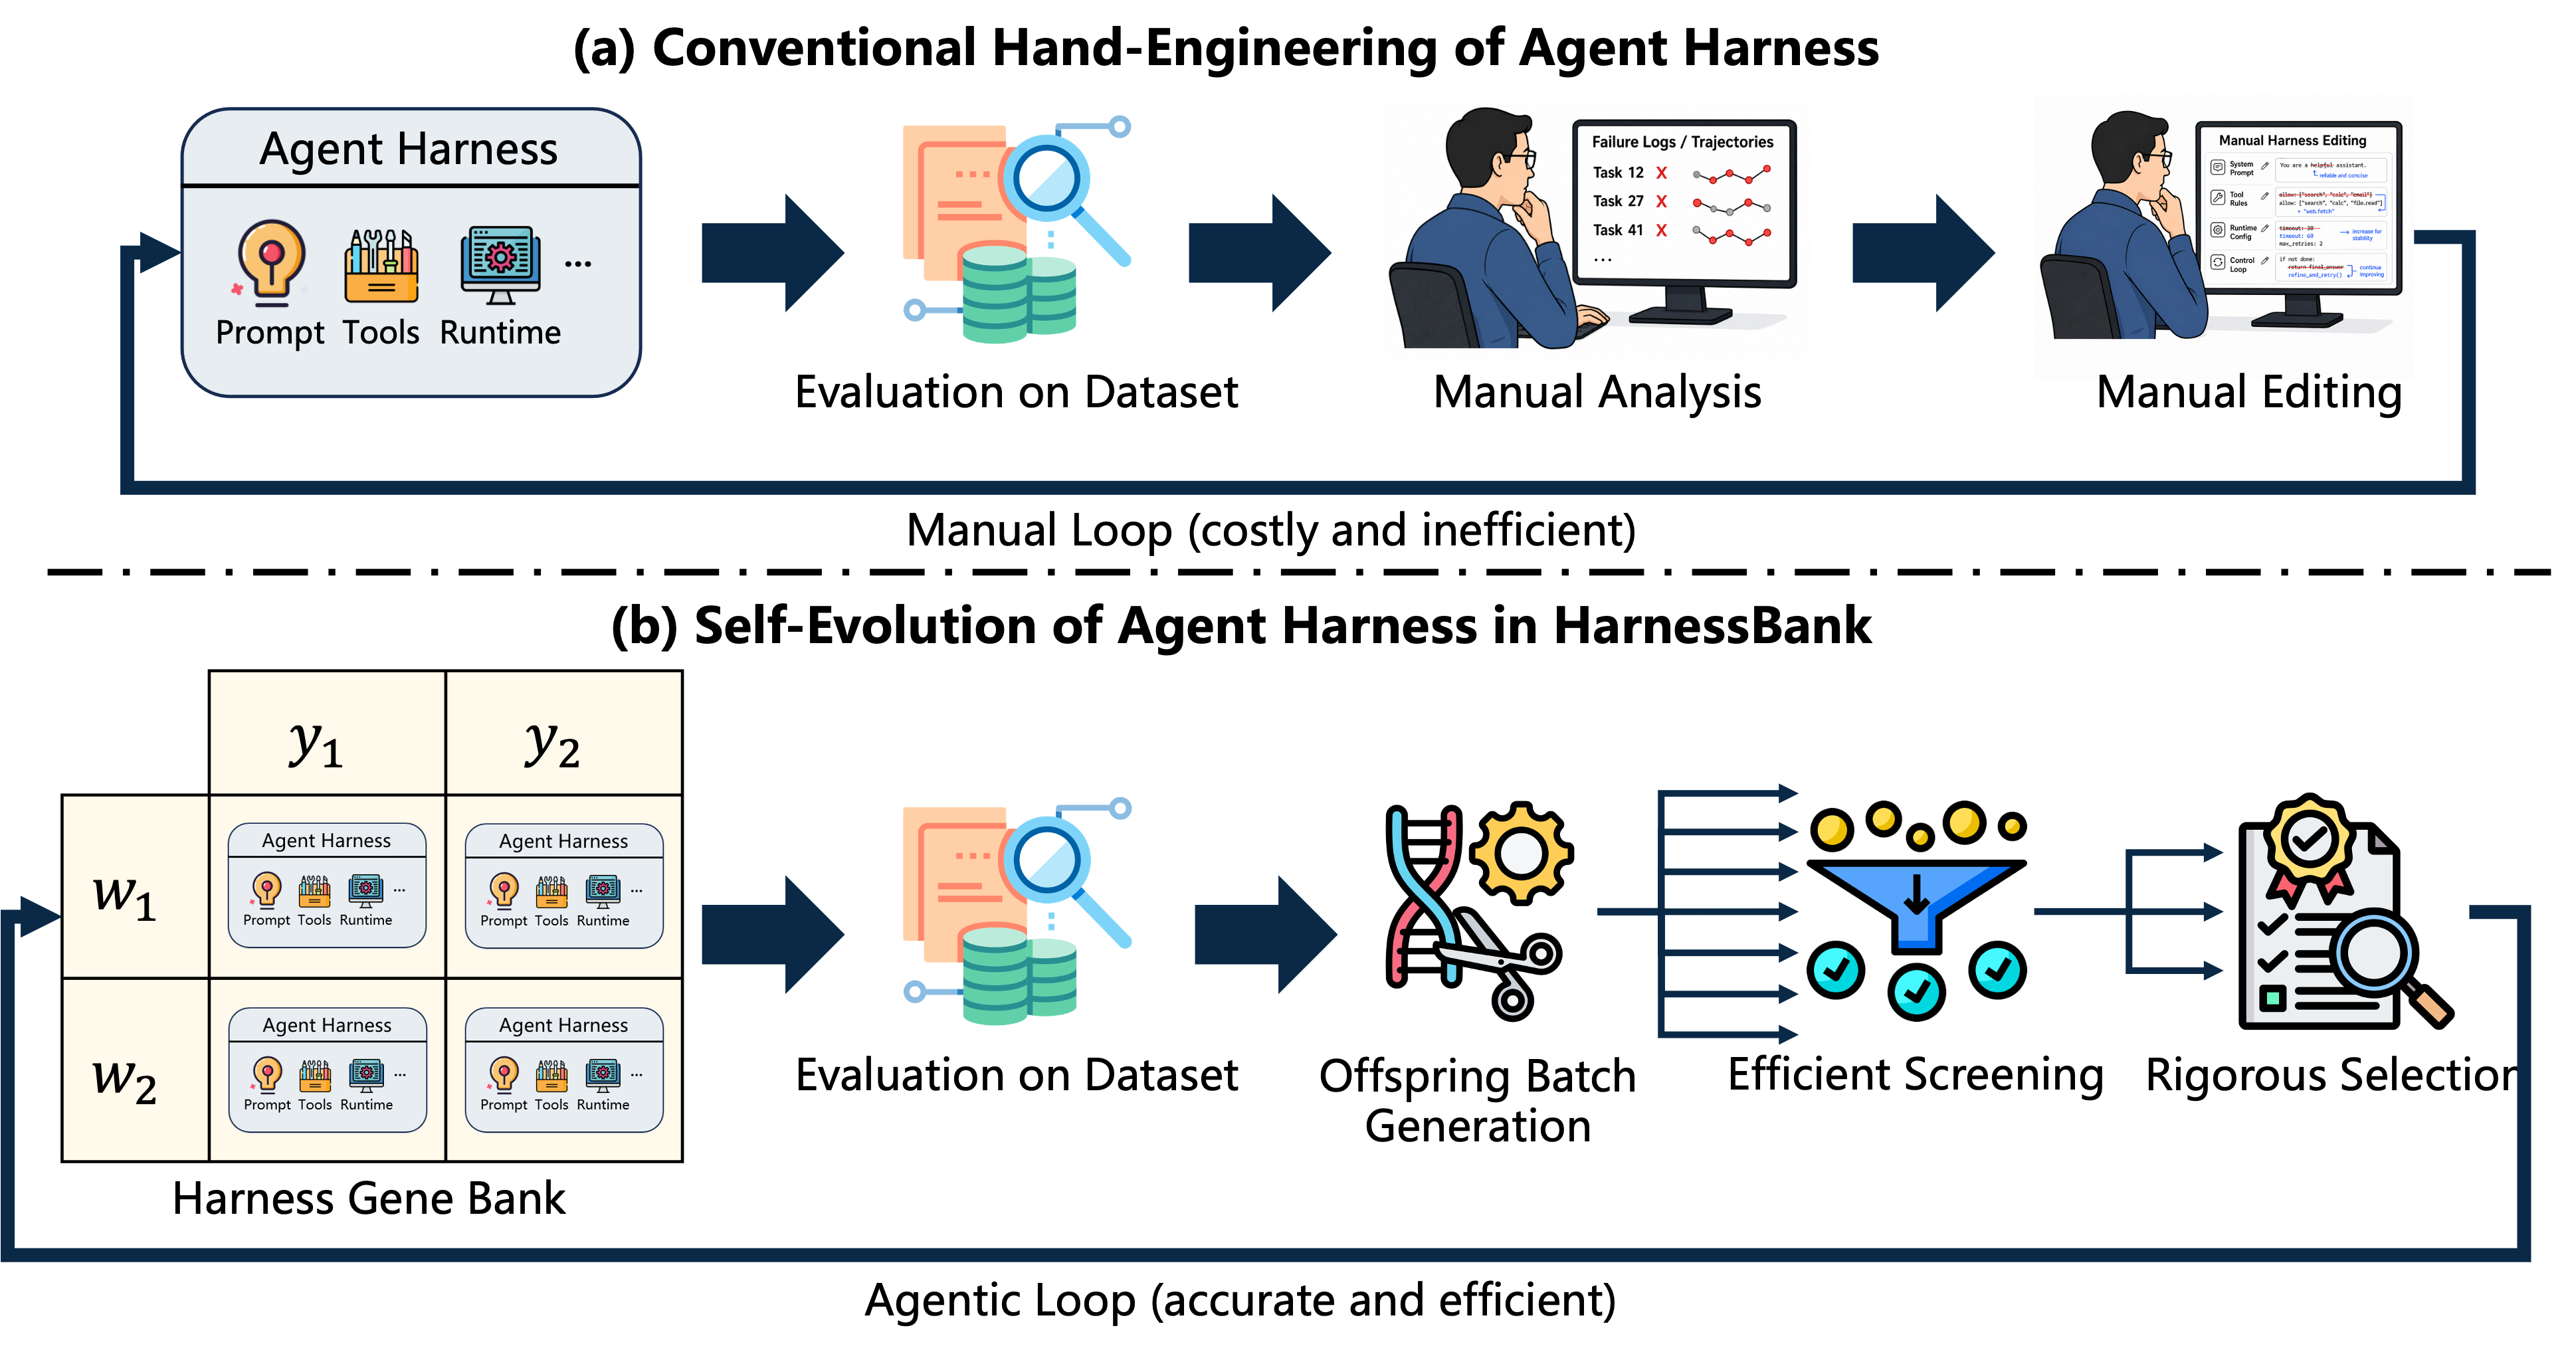
\includegraphics[width=1\linewidth]{figures/fig1.png}
  \caption{Conventional Hand-Engineering vs. Agent-Harness Self-Evolution: manual loop of agent harness development is costly and inefficient while self-evolution of agent harness in HarnessBank is accurate and efficient.}
  \label{fig:fig}
\end{figure}

Recent studies have begun to automate this process by allowing agents to inspect execution trajectories, propose harness modifications, and retain modifications that appear beneficial~\citep{zhang2026selfharness,chen2026harnessfix}. These studies demonstrate that harness-level adaptation can improve agent performance without model fine-tuning.
%
However, existing approaches commonly follow a relatively greedy evolution procedure in which a small number of locally promising edits are repeatedly promoted \citep{lin2026ahe,chen2026harnessx}.
%
Such procedures provide limited support for preserving structurally different solutions or combining complementary improvements, and may consequently collapse toward a narrow class of safe modifications, particularly prompt-level edits.
%
Moreover, for efficiency, candidates are often selected using single-run improvements, non-regression criteria, or model-predicted utility, without explicitly verifying whether the proposed mechanism is activated or whether the observed gain exceeds execution noise~\citep{ursekar2026vero,hambardzumyan2026aira2}.
%
These limitations make current self-evolution procedures susceptible to search collapse, task-specific overfitting, and unverifiable performance gains.


Based on the above observations, achieving trustworthy agent-harness self-evolution presents two fundamental challenges. 
%
\textbf{First, harness evolution requires structured exploration over a large and heterogeneous modification space.}
%
A harness may be improved through changes to prompts, injected knowledge, runtime control logic, recovery mechanisms, tool interfaces, or numerical configurations, yielding an effectively unbounded set of possible designs.
%
Greedy evolution tends to repeatedly exploit the current best candidate and gradually collapse toward conservative, incremental modifications after more ambitious offspring fail~\citep{ursekar2026vero}.
%
It may also retain patches that memorize particular training tasks rather than correct recurring failure mechanisms.
%
A successful self-evolution procedure must therefore preserve high-performing but semantically distinct harnesses, while enabling their useful mechanisms to be reinvented and recombined across generations.
%
\textbf{Second, identifying genuinely improved harnesses is both difficult and computationally expensive.}
%
Evaluating every offspring harness over the complete training set requires substantial agent rollouts, yet inexpensive evaluations on small task subsets can be unreliable.
%
Agent outcomes fluctuate across repeated executions, particularly on borderline tasks, while sandbox crashes, verifier timeouts, and other infrastructure artifacts may be incorrectly attributed to harness modifications.
%
Furthermore, an apparently successful patch may never activate during execution, or may overfit the tasks used to select it.
%
Trustworthy evolution therefore requires an efficient screening protocol that distinguishes functional and reproducible improvements from inactive mechanisms, stochastic variation, and evaluation artifacts.

To address these challenges, we introduce \textbf{HarnessBank}, a trustworthy agent-harness self-evolution framework that pairs a \emph{task agent} with a separate \emph{evolver agent}.
%
The task agent executes environment tasks under its current harness, whereas the evolver analyzes execution trajectories, diagnoses recurring failure mechanisms, and generates offspring harnesses without modifying the task model's parameters.
%
To prevent search collapse, HarnessBank introduces a \emph{Harness Gene Bank} that preserves high-performing harnesses across semantic coordinates.
%
Each bank cell is indexed by \emph{where} a harness modification acts and \emph{why} it is introduced, corresponding respectively to the modified harness component and the targeted failure pathology.
%
Harnesses targeting different failure mechanisms remain available for subsequent evolution.
%
The evolver can consequently produce offspring either by reinventing a mechanism from failure trajectories or by recombining compatible mechanisms preserved in different cells.
%
Quality-biased parent selection exploits the strongest discovered lineage, while the semantic bank retains complementary solutions that would otherwise be discarded by conventional greedy evolution.
%
To efficiently and reliably select offspring harnesses, HarnessBank further introduces \emph{Gated Harness Screening}.
%
Rather than immediately evaluating every offspring on the complete training set, HarnessBank first evaluates candidates on a sampled task subset and applies four sequential gates.
%
A validity gate excludes outcomes corrupted by infrastructure failures; an activation gate verifies that the proposed modification actually executes; a paired significance gate tests whether the observed gain is distinguishable from task-level variation; and a gain gate requires the candidate to outperform its parent.
%
Candidates that pass the screening procedure are subsequently evaluated on the complete training set before competing for admission to the Harness Gene Bank.
%
Across seven diverse agent benchmarks, HarnessBank consistently improves the performance of frozen task agents, with gains ranging from $5.1\%$ to $15.4\%$.


Our main contributions are summarized as follows:

\begin{itemize}[leftmargin=*]
\item We propose \textbf{HarnessBank}, an end-to-end framework for trustworthy agent-harness self-evolution. HarnessBank pairs a task agent with a separate evolver agent that iteratively diagnoses execution failures, generates candidate harnesses, and verifies their improvements without updating the underlying model parameters.

\item To mitigate search collapse and task-specific overfitting, we introduce a \textbf{Harness Gene Bank} that organizes high-performing harnesses using semantic coordinates. By preserving harnesses that address distinct failure pathologies, the gene bank supports both failure-guided reinvention and cross-cell recombination, enabling structured exploration beyond greedy optimization of a single harness lineage.

\item To efficiently and reliably identify improved harnesses, we propose \textbf{Gated Harness Screening}, which evaluates candidates on a sampled training subset through sequential checks of evaluation validity, mechanism activation, statistical significance, and performance gain. Only candidates that pass all gates undergo full training-set evaluation and compete for admission to the Harness Gene Bank.

\item  Experiments across seven diverse agent benchmarks demonstrate that HarnessBank consistently improves task agents, with performance gains ranging from $5.1\%$ to $15.4\%$. Cross-model experiments further show that the evolved harnesses are model-specific rather than universally optimal, indicating that the transferable capability lies in the failure-diagnosis, structured-search, and verification process.
\end{itemize}